\section{Control loop}
% Control Loop (differences between the two, from where they start to where they close, freuqency for the various elements)

\begin{frame}{Control loop}

    Close-loop approach to \textbf{lock the LO\footnotemark[1] frequency to the atomic transition}.

    \vspace{10pt}

    \begin{columns}[c, onlytextwidth]

        \begin{column}{0.6\textwidth}

            \begin{figure}
                \centering
                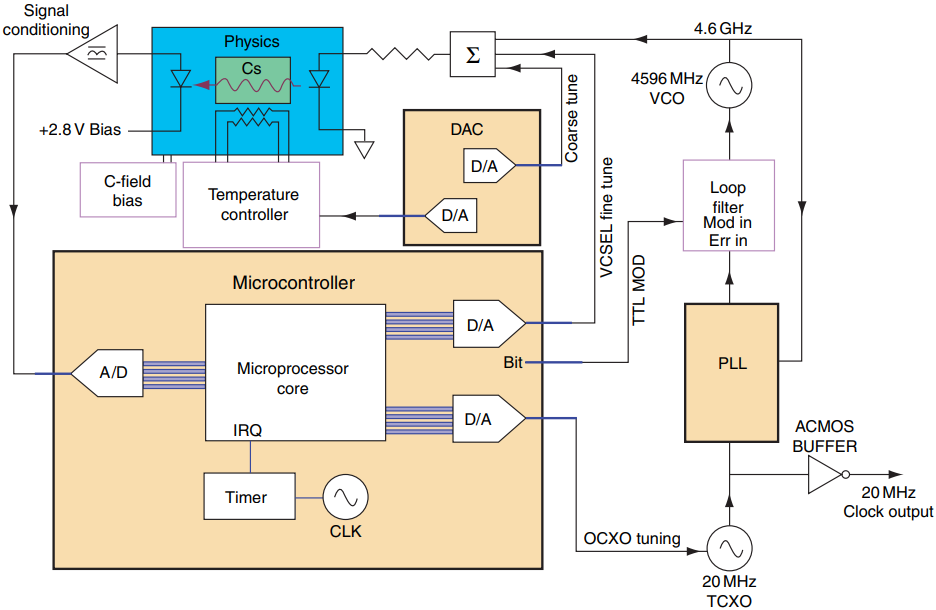
\includegraphics[width=0.9\textwidth]{img/control-loop.png}
                \caption{Control loop block diagram.}
            \end{figure}

        \end{column}

        \begin{column}{0.4\textwidth}

            PI\footnotemark[2] controllers are used to minimize the error between the target and the actual value.

            \vspace{10pt}

            Indispensable targets:

            \begin{itemize}
                \item LO frequency
                \item Laser frequency
                \item Laser temperature
                \item Cell temperature
            \end{itemize}

        \end{column}

    \end{columns}

    \footnotetext[1]{LO: Local Oscillator}
    \footnotetext[2]{PI: Proportional-Integral}

\end{frame}



\begin{frame}{Electronics}

    \begin{columns}[c, onlytextwidth]

        \begin{column}{0.6\textwidth}

            Here are some possible problematic areas:

            \begin{itemize}
                \item Stability in voltage and current provided to VCO and VCSEL (highly sensitive components)
                \item Cross-talk between different control loops
                \item Noise from the electronics
                \item Power consumption ($\approx 10\%$ of the total)
            \end{itemize}

        \end{column}

        \hfill

        \begin{column}{0.35\textwidth}

            \begin{figure}
                \centering
                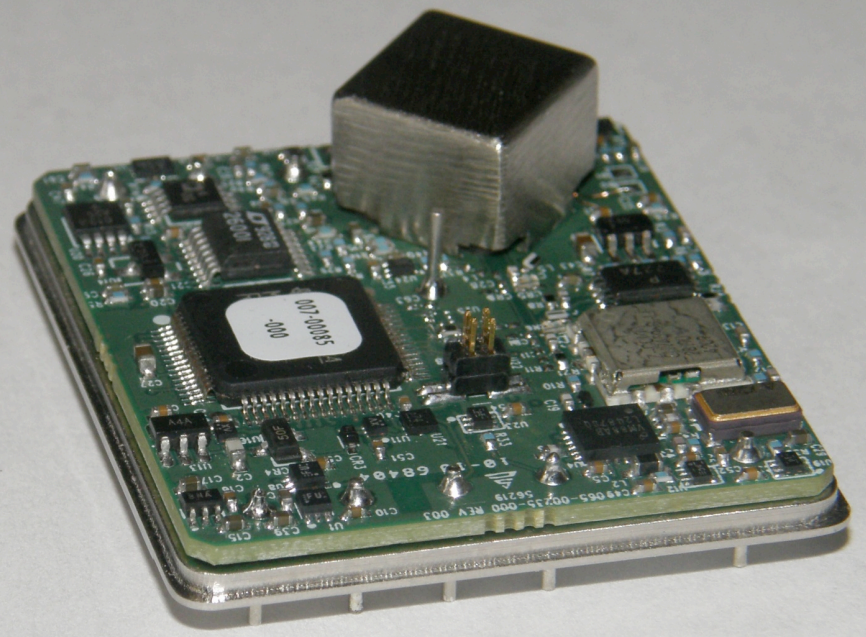
\includegraphics[width=\textwidth]{img/electronics-CSCA-SA45s.png}
                \caption{CSAC SA.45s from Microchip.}
            \end{figure}

        \end{column}

    \end{columns}

\end{frame}